%==========================================
%
% Sibgrapi 2021 paper template
% Example of IEEEtran.cls
%
%==========================================

% *** Authors should verify (and, if needed, correct) their LaTeX system  ***
% *** with the testflow diagnostic prior to trusting their LaTeX platform ***
% *** with production work. The IEEE's font choices and paper sizes can   ***
% *** trigger bugs that do not appear when using other class files.       ***                          ***
% The testflow support page is at:
% http://www.michaelshell.org/tex/testflow/

\RequirePackage[OT1]{fontenc}
\documentclass[10pt,conference]{IEEEtran}


% Some very useful LaTeX packages include:
% (uncomment the ones you want to load)


% *** MISC UTILITY PACKAGES ***
%
%\usepackage{ifpdf}
% Heiko Oberdiek's ifpdf.sty is very useful if you need conditional
% compilation based on whether the output is pdf or dvi.
% usage:
% \ifpdf
%   % pdf code
% \else
%   % dvi code
% \fi
% The latest version of ifpdf.sty can be obtained from:
% http://www.ctan.org/pkg/ifpdf
% Also, note that IEEEtran.cls V1.7 and later provides a builtin
% \ifCLASSINFOpdf conditional that works the same way.
% When switching from latex to pdflatex and vice-versa, the compiler may
% have to be run twice to clear warning/error messages.






% *** CITATION PACKAGES ***
%
\usepackage{cite}
% cite.sty was written by Donald Arseneau
% V1.6 and later of IEEEtran pre-defines the format of the cite.sty package
% \cite{} output to follow that of the IEEE. Loading the cite package will
% result in citation numbers being automatically sorted and properly
% "compressed/ranged". e.g., [1], [9], [2], [7], [5], [6] without using
% cite.sty will become [1], [2], [5]--[7], [9] using cite.sty. cite.sty's
% \cite will automatically add leading space, if needed. Use cite.sty's
% noadjust option (cite.sty V3.8 and later) if you want to turn this off
% such as if a citation ever needs to be enclosed in parenthesis.
% cite.sty is already installed on most LaTeX systems. Be sure and use
% version 5.0 (2009-03-20) and later if using hyperref.sty.
% The latest version can be obtained at:
% http://www.ctan.org/pkg/cite
% The documentation is contained in the cite.sty file itself.






% *** GRAPHICS RELATED PACKAGES ***
%
\ifCLASSINFOpdf
   \usepackage[pdftex]{graphicx}
  % declare the path(s) where your graphic files are
   \graphicspath{{figs/}}
  % and their extensions so you won't have to specify these with
  % every instance of \includegraphics
   \DeclareGraphicsExtensions{.pdf,.jpeg,.png}
\else
  % or other class option (dvipsone, dvipdf, if not using dvips). graphicx
  % will default to the driver specified in the system graphics.cfg if no
  % driver is specified.
   \usepackage[dvips]{graphicx}
  % declare the path(s) where your graphic files are
   \graphicspath{{../figs/}}
  % and their extensions so you won't have to specify these with
  % every instance of \includegraphics
   \DeclareGraphicsExtensions{.eps}
\fi
% graphicx was written by David Carlisle and Sebastian Rahtz. It is
% required if you want graphics, photos, etc. graphicx.sty is already
% installed on most LaTeX systems. The latest version and documentation
% can be obtained at: 
% http://www.ctan.org/pkg/graphicx
% Another good source of documentation is "Using Imported Graphics in
% LaTeX2e" by Keith Reckdahl which can be found at:
% http://www.ctan.org/pkg/epslatex
%
% latex, and pdflatex in dvi mode, support graphics in encapsulated
% postscript (.eps) format. pdflatex in pdf mode supports graphics
% in .pdf, .jpeg, .png and .mps (metapost) formats. Users should ensure
% that all non-photo figures use a vector format (.eps, .pdf, .mps) and
% not a bitmapped formats (.jpeg, .png). The IEEE frowns on bitmapped formats
% which can result in "jaggedy"/blurry rendering of lines and letters as
% well as large increases in file sizes.
%
% You can find documentation about the pdfTeX application at:
% http://www.tug.org/applications/pdftex





% *** MATH PACKAGES ***
%
\usepackage[cmex10]{amsmath}
% A popular package from the American Mathematical Society that provides
% many useful and powerful commands for dealing with mathematics.
%
% Note that the amsmath package sets \interdisplaylinepenalty to 10000
% thus preventing page breaks from occurring within multiline equations. Use:
\interdisplaylinepenalty=2500
% after loading amsmath to restore such page breaks as IEEEtran.cls normally
% does. amsmath.sty is already installed on most LaTeX systems. The latest
% version and documentation can be obtained at:
% http://www.ctan.org/pkg/amsmath
\usepackage{amsthm}
\newtheorem{definition}{Definition}




% *** SPECIALIZED LIST PACKAGES ***
%
\usepackage{algorithmic}
% algorithmic.sty was written by Peter Williams and Rogerio Brito.
% This package provides an algorithmic environment fo describing algorithms.
% You can use the algorithmic environment in-text or within a figure
% environment to provide for a floating algorithm. Do NOT use the algorithm
% floating environment provided by algorithm.sty (by the same authors) or
% algorithm2e.sty (by Christophe Fiorio) as the IEEE does not use dedicated
% algorithm float types and packages that provide these will not provide
% correct IEEE style captions. The latest version and documentation of
% algorithmic.sty can be obtained at:
% http://www.ctan.org/pkg/algorithms
% Also of interest may be the (relatively newer and more customizable)
% algorithmicx.sty package by Szasz Janos:
% http://www.ctan.org/pkg/algorithmicx




% *** ALIGNMENT PACKAGES ***
%
\usepackage{array}
% Frank Mittelbach's and David Carlisle's array.sty patches and improves
% the standard LaTeX2e array and tabular environments to provide better
% appearance and additional user controls. As the default LaTeX2e table
% generation code is lacking to the point of almost being broken with
% respect to the quality of the end results, all users are strongly
% advised to use an enhanced (at the very least that provided by array.sty)
% set of table tools. array.sty is already installed on most systems. The
% latest version and documentation can be obtained at:
% http://www.ctan.org/pkg/array


% IEEEtran contains the IEEEeqnarray family of commands that can be used to
% generate multiline equations as well as matrices, tables, etc., of high
% quality.




% *** SUBFIGURE PACKAGES ***
\ifCLASSOPTIONcompsoc
  \usepackage[caption=false,font=normalsize,labelfont=sf,textfont=sf]{subfig}
\else
  \usepackage[caption=false,font=footnotesize]{subfig}
\fi
% subfig.sty, written by Steven Douglas Cochran, is the modern replacement
% for subfigure.sty, the latter of which is no longer maintained and is
% incompatible with some LaTeX packages including fixltx2e. However,
% subfig.sty requires and automatically loads Axel Sommerfeldt's caption.sty
% which will override IEEEtran.cls' handling of captions and this will result
% in non-IEEE style figure/table captions. To prevent this problem, be sure
% and invoke subfig.sty's "caption=false" package option (available since
% subfig.sty version 1.3, 2005/06/28) as this is will preserve IEEEtran.cls
% handling of captions.
% Note that the Computer Society format requires a larger sans serif font
% than the serif footnote size font used in traditional IEEE formatting
% and thus the need to invoke different subfig.sty package options depending
% on whether compsoc mode has been enabled.
%
% The latest version and documentation of subfig.sty can be obtained at:
% http://www.ctan.org/pkg/subfig




% *** FLOAT PACKAGES ***
%
%\usepackage{fixltx2e}
% fixltx2e, the successor to the earlier fix2col.sty, was written by
% Frank Mittelbach and David Carlisle. This package corrects a few problems
% in the LaTeX2e kernel, the most notable of which is that in current
% LaTeX2e releases, the ordering of single and double column floats is not
% guaranteed to be preserved. Thus, an unpatched LaTeX2e can allow a
% single column figure to be placed prior to an earlier double column
% figure.
% Be aware that LaTeX2e kernels dated 2015 and later have fixltx2e.sty's
% corrections already built into the system in which case a warning will
% be issued if an attempt is made to load fixltx2e.sty as it is no longer
% needed.
% The latest version and documentation can be found at:
% http://www.ctan.org/pkg/fixltx2e


%\usepackage{stfloats}
% stfloats.sty was written by Sigitas Tolusis. This package gives LaTeX2e
% the ability to do double column floats at the bottom of the page as well
% as the top. (e.g., "\begin{figure*}[!b]" is not normally possible in
% LaTeX2e). It also provides a command:
%\fnbelowfloat
% to enable the placement of footnotes below bottom floats (the standard
% LaTeX2e kernel puts them above bottom floats). This is an invasive package
% which rewrites many portions of the LaTeX2e float routines. It may not work
% with other packages that modify the LaTeX2e float routines. The latest
% version and documentation can be obtained at:
% http://www.ctan.org/pkg/stfloats
% Do not use the stfloats baselinefloat ability as the IEEE does not allow
% \baselineskip to stretch. Authors submitting work to the IEEE should note
% that the IEEE rarely uses double column equations and that authors should try
% to avoid such use. Do not be tempted to use the cuted.sty or midfloat.sty
% packages (also by Sigitas Tolusis) as the IEEE does not format its papers in
% such ways.
% Do not attempt to use stfloats with fixltx2e as they are incompatible.
% Instead, use Morten Hogholm'a dblfloatfix which combines the features
% of both fixltx2e and stfloats:
%
% \usepackage{dblfloatfix}
% The latest version can be found at:
% http://www.ctan.org/pkg/dblfloatfix




% *** PDF, URL AND HYPERLINK PACKAGES ***
%
\usepackage{url}
% url.sty was written by Donald Arseneau. It provides better support for
% handling and breaking URLs. url.sty is already installed on most LaTeX
% systems. The latest version and documentation can be obtained at:
% http://www.ctan.org/pkg/url
% Basically, \url{my_url_here}.




% *** Do not adjust lengths that control margins, column widths, etc. ***
% *** Do not use packages that alter fonts (such as pslatex).         ***
% There should be no need to do such things with IEEEtran.cls V1.6 and later.
% (Unless specifically asked to do so by the journal or conference you plan
% to submit to, of course. )


% correct bad hyphenation here
% \hyphenation{op-tical net-works semi-conduc-tor}

%------------------------------------------------------------------------- 
% change the % on next lines to produce the final camera-ready version 
\newcommand{\cmtid}{11}

\newif\iffinal

% \finalfalse
\finaltrue

\usepackage[switch]{lineno}

\iffinal
    \usepackage[final]{verlab}
\else
    \usepackage[highlight]{verlab}
    \linenumbers
\fi

\usepackage{graphicx}
\usepackage{cite}

\usepackage[hidelinks]{hyperref}
\usepackage[inline]{enumitem}
\usepackage{url}
\usepackage{subfig}

\usepackage[cmex10]{amsmath}
\usepackage{amsthm}

% Section: Standardized operator names.

\DeclareMathOperator{\Gaussian}{Gaussian}
\DeclareMathOperator{\Grayscale}{Grayscale}
\DeclareMathOperator{\Sketch}{Sketch}

\DeclareMathOperator{\MSDSSIM}{MS-DSSIM}
\DeclareMathOperator{\MSSSIM}{MS-SSIM}
\DeclareMathOperator{\DSSIM}{DSSIM}
\DeclareMathOperator{\SSIM}{SSIM}
\DeclareMathOperator{\PSNR}{PSNR}
\DeclareMathOperator{\MSE}{MSE}
\DeclareMathOperator{\MAE}{MAE}
\DeclareMathOperator{\SSIMCS}{CS}
\DeclareMathOperator{\SSIML}{L}

\DeclareMathOperator{\MixedGradientError}{MixGE}

% Section: Tables

\usepackage{booktabs}
\usepackage{multirow}
\usepackage{makecell}

\renewcommand\theadfont{\bfseries}


\newcommand{\orcid}[1]{\hspace{1px}\raisebox{2px}{\href{https://orcid.org/#1}{\includegraphics[scale=0.04]{figs/ORCIDiD.pdf}}}}

\begin{document}

\title{Evaluating Loss Functions for Illustration Super-Resolution Neural Networks}


\author{
  \IEEEauthorblockN{Raphael Nepomuceno\orcid{0000-0003-4923-7896
    } and Michel M. Silva\orcid{0000-0002-2499-9619}}
  \IEEEauthorblockA{Department of Informatics, Universidade Federal de Vi\c{c}osa (DPI-UFV), Vi\c{c}osa -- MG, 36.570-900, Brazil\\
    E-mails: \{raphael.nepomuceno, michel.m.silva\}@ufv.br
  }
}

\maketitle

\begin{abstract}
  As display technologies evolve and high-resolution screens become more available, the desirability of images and videos with high perceptual quality grows in order to properly utilize such advances. At the same time, the market for illustrated mediums, such animations and comics, has been in steady growth over the past years. Based on these observations, we were motivated to explore the super-resolution task in the niche of drawings. In absence of original high-resolution imagery, it is necessary to use approximate methods, such as interpolation algorithms, to enhance low-resolution media. Such methods, however, can produce undesirable artifacts in the reconstructed images, such as blurring and edge distortions. Recent works have successfully applied deep learning to this task, but such efforts are often aimed at real-world images and do not take in account the specifics of illustrations, which emphasize lines and employ simplified patterns rather than complex textures, which in turn makes visual artifacts introduced by algorithms easier to spot. With these differences in mind, we evaluated the effects of the choice of loss functions in order to obtain accurate and perceptually pleasing results in the super-resolution task for comics, cartoons, and other illustrations. Experimental evaluations have shown that a loss function based on edge detection performs best in this context among the evaluated functions, though still showing room for further improvements.

% As display technologies evolve and high-resolution screens become more available, the desirability of images and videos with high perceptual quality grows in order to properly utilize such advances. \todo{Falar do aumento de conteudo de animacoes, e da grande atencao que esta sendo dada aos quadrinhos e manga. Deixar claro aqui que o trabalho eh sobre animacoes} In absence of original high-resolution imagery, it is necessary to use approximate methods, such as interpolation algorithms, to enhance low-resolution media. \todo{Qual o problema em resolver usando metodos aproximados?} While recent works have successfully applied deep learning to this task, such efforts are often aimed at real-world pictures and do not consider the specifics of illustrations, which emphasize lines and employ simplified patterns rather than complex textures, thereby emphasizing imperfections originated from the process \todo{não entendi essa parte após a vírgula}. With these differences in mind, we evaluated the effects of the choice of loss functions in order to obtain accurate and perceptually pleasing results in the task of \review{super-resolving - esta correto?} comics, cartoons, and other illustrations. Experimental evaluations have shown that a loss function based on edge detection performs best in this context among the evaluated functions, though still showing room for further improvements.
\end{abstract}

% \IEEEpeerreviewmaketitle

\section{Introduction}

Nowadays, high-definition screens are becoming increasingly available due to advances in display technologies: statistics show a nine fold growth in the number of ultra-high-definition televisions from $2014$ to $2019$~\cite{statista2019tv}. To make the best use of high-definition displays, the availability of high-resolution imagery is desirable. However, while new content may be produced in high-resolution, previously recorded media may only be available in low-resolution.

Enlarging images requires the use of some method to fill in pixels with unknown values. The most naive method, referred to as nearest neighbor interpolation, is to repeat the intensity of the closest known pixel. However, this method introduces artifacts on the image, creating aliasing. A more elaborated method to fill in the unknown values is to interpolate the intensity based on the neighbors value and a polynomial function: \eg, linear and bicubic interpolation. The choice of the interpolation method also impacts the perceptual quality of the result by potentially producing unwanted artifacts: in this case, there is a loss in the definition of the edges as the image becomes blurry~\cite{gonzalez2018}. Figure~\ref{fig:interpolation} exemplifies the artifacts introduced by the nearest neighbor and bicubic interpolation methods.

\begin{figure}[t]
  \centering

  \subfloat[Ground~Truth\label{figure:interpolation/truth}]{ \includegraphics[width=0.3\linewidth]{figs/interpolation/original} }
  \hfill
  \subfloat[Nearest neighbor interpolation\label{figure:interpolation/nearest}]{ \includegraphics[width=0.3\linewidth]{figs/interpolation/nearest} }
  \hfill
  \subfloat[Bicubic interpolation\label{figure:interpolation/bicubic}]{ \includegraphics[width=0.3\linewidth]{figs/interpolation/cubic} }

  \caption{
    Examples of distortions produced by interpolation methods when applied to a low-resolution version of image~\ref{figure:interpolation/truth}. Regions outlined in magenta are magnified to aid the comparison between methods. The edges in image \ref{figure:interpolation/nearest} have aliasing artifacts not present in the Ground~Truth. In the result of the interpolation method \ref{figure:interpolation/bicubic}, it is possible to observe the blur along the edges. The Ground~Truth image is from the SYNLA dataset~\cite{synla}.
    \label{fig:interpolation}}
\end{figure}

Single-Image Super-Resolution (SISR) is a classical task in computer vision of recovering a high-resolution image from a single low-resolution sample. It is inherently a ill-posed problem, as several possible solutions exist for a given low-resolution image~\cite{dong2015image}.
Due to the details present in high-resolution images with high perceptual quality, the task is widely used in works involving high-definition television, medical, satellite and security imagery~\cite{shi2016realtime, yang2019deep}.

One of the previous representative solutions for this problem employed a pipeline based on sparse coding pipeline with steps such as patch-extraction, dictionary look-ups and reconstruction in order to perform this task \cite{yang2008image,yang2010image}. However, it was shown that the process could be made more efficient, and potentially more accurate, by employing Convolutional Neural Networks (CNNs) with internal layers equivalent to such steps~\cite{dong2015image}.

In fact, CNNs achieved memorable results in the task of creating super-resolution images~\cite{shi2016realtime, dong2015image, ledig2017photorealistic, lim2017enhanced}. However, their application is focused on real world images. Therefore, one of the media type often reproduced in the high-quality screens, the illustrations, are underrepresented in the deep learning literature.

Illustrations, \ie images from comic books, manga, cartoons and anime, are produced by an entirely different process from photography and generally focus only on salient details while abstracting the rest: edges are overly emphasized and complex textures are often replaced with flat regions or simplified patterns. In applications such as style transfer, these intrinsic difference causes the neural network to produce undesirable artifacts likened to watercolor paintings, where noisy transition textures are generated instead of the expected simplified patterns~\cite{danbooru2020}. The proposed work explores the application of deep learning techniques --- specifically, CNNs --- to the problem of single-image super resolution within the niche of illustrations, which potential applications include enhancing drawing, comics or --- when combined with video processing techniques --- animations~\cite{dandere2x}.

The main contribution of this work is a quantitative, through the SSIM and PSNR metrics, and qualitative evaluation of four loss functions in order to determine which produces the most accurate and perceptually pleasing images in the SISR task. \adding{Furthermore, we evaluate whether using a larger neural network impacts the ordering of the best to worst loss functions.}

\begin{figure*}[t]
  \includegraphics[width=\linewidth]{figs/3rd-party/shi2016realtime/networkstructure.jpg}
  \caption{Architecture overview of the ESPCN~\cite{shi2016realtime} network. Our application of the architecture differs from the original by inserting a normalization layer after the input and by using RGB images from end to end. Source: Shi~\etal~\cite{shi2016realtime}}
  \label{figure:espcn}
\end{figure*}
\section{Related Work}

In this section, we present an overview of the Single-Image Super-Resolution (SISR) area by exploring remarkable works. For the sake of clarity, we divide the works in the section related to CNN architectures, quality metrics, and loss functions applied in the SISR problem.

\subsection{Super-resolution neural networks}

The concept of Convolutional Neural Networks has been around since the late 1980s~\cite{lecun1989backpropagation}, with its resurgence in recent years justified by advances in hardware and algorithms and by the favorable results exhibited in tasks such as image classification and object recognition~\cite{dong2015image,yang2019deep}.

A breakthrough in the application of deep learning for single-image super-resolution was the SRCNN~\cite{dong2015image}, which first scaled the input images with the bicubic interpolation and then forwarded their Y-channel through three convolutional layers. This approach can be seen as using a neural network to reduce the artifacts introduced by the bicubic method in the resulting image. The results achieved by the approach either surpassed or matched the state of the art at the time.

Shi~\etal proposed the Efficient Sub-Pixel Convolutional Neural network (ESPCN)~\cite{shi2016realtime} architecture, which has shown superior results over the SRCNN while being more time efficient and with fewer learnable weights. \adding{This was enabled by the removal of the bicubic interpolation step, which increased feature map sizes while not producing an equivalent amount of additional information, and the use of the sub-pixel convolution layer, depicted in Figure~\ref{figure:espcn}, as the network output.}

Deeper architectures, such as SRResNet~\cite{ledig2017photorealistic}, EDSR~\cite{lim2017enhanced} and RDN~\cite{zhang2018residual}, have been enabled by the use of residual networks~\cite{he2016deep}, which address the vanishing gradients problem~\cite{bengio1994learning}.

Haris~\etal~\cite{haris2018deep} proposed an iterative up and downsampling method with units combining intermediate features to error maps calculated by upsampling the error in an internal input reconstruction pipeline.

\subsection{Loss functions for image reconstruction}

The loss function serves as the objective in the deep learning optimization process, guiding its training and, in image reconstruction tasks, determining how to compare a synthesized sample to its ground truth~\cite{zhao2016loss}. Given the differences between illustrations and photographs, we are interested in examining the effects that the choice of a loss function on the characteristics of the reconstructed images. The focus of this work is in the analysis of four loss functions: Mean Squared Error, Mean Absolute Error, the usage of the Structural Similarity Index Measure as a loss function~\cite{zhao2016loss}, and, based on the emphasis on contours that illustrations commonly exhibit, a mixed loss function which accounts for image gradients through the Sobel operator~\cite{lu2019single}.

The mean squared error (MSE) loss is considered a popular choice \cite{zhao2016loss}, being employed in the works we build upon \cite{dong2015image,shi2016realtime}. The use of mean absolute error (MAE) was proposed as an attempt to overcome limitations of the MSE, said to produce splotchy artifacts \cite{zhao2016loss}. Despite the MAE providing improvements over the MSE, its results were said to be sub-optimal, leading to the exploration of other loss functions \cite{zhao2016loss}. The structural similarity index measure (SSIM)~\cite{wang2004image} is a metric motivated by the human visual perception, which evaluates images accounting for perceived changes in structural information. Zhao~\etal proposed the use of the SSIM \adding{and the multi-scale SSIM} as loss functions for image restoration neural networks.

Alternatives have been proposed in order to produce images with higher perceptual quality for humans. Johnson~\etal proposed to use a feature extractor from a classifier, \eg, VGG-16~\cite{simonyan2015deep}, to describe the ground truth and reconstructed image, and then calculate the distance between the feature maps. The authors demonstrate that this perceptual loss embed domain knowledge in the training process~\cite{johnson2016perceptual}. Ledig~\etal~\cite{ledig2017photorealistic} introduced the use of Generative Adversarial Networks (GANs)~\cite{goodfellow2014generative} for SISR in order to produce photo-realistic images.

Given that illustrations place emphasis on lines, a method that optimizes for that should intuitively perform better. The use of an edge detection operator provides another means of embedding such domain knowledge in the context of illustrations. To that end, we explored the mixed gradient error, which is composed by MSE and a weighted mean gradient error~\cite{lu2019single}, calculated using the classic edge detection filter proposed by Sobel~\cite{kanopoulos1988design}.
\adding{A loss function based on the pencil sketch border detection filter, which, unlike the Sobel filter, preserves depth information}~\cite{galindo2019image}\adding{, was also explored.}

\subsection{Evaluating perceptual quality}

The structural similarity index measure (SSIM) and peak signal-to-noise ratio (PSNR) are widely used metrics for quantitatively estimating the effectiveness of image reconstruction methods \cite{dong2015image,shi2016realtime,zhao2016loss,lu2019single}. However, their adequacy for the human perception has been questioned, with works exhibiting restored images with better perceptual quality despite lower metric scores \cite{johnson2016perceptual,ledig2017photorealistic}. Thus, we also direct our focus in qualitative comparisons across loss functions.
\section{Methodology}

Our work consisted in evaluating the effects of the loss function in the training of CNNs for the single-image super-resolution task for illustrations.
Each loss was evaluated by training our chosen neural network architectures from scratch using an illustration dataset, then we performed quantitative and qualitative analysis on their outputs.
In this section, we present how we carried the training and the analysis of the CNN models.

% \subsection{\cutoff{Neural network architecture}}
% \label{sec:metodologia-cnn}


% We base our methodology upon the ESPCN~\cite{shi2016realtime} CNN architecture, presented in Figure~\ref{figure:espcn}. The choice of a shallower network architecture over the more recent deep residual networks~\cite{ledig2017photorealistic,lim2017enhanced} is based on the goal of this work of making relative evaluations of loss functions, under the assumption that such relationships would be maintained if reevaluated on more complex networks. Thus, we default to training the simpler architecture, aiming faster experimentation cycles.

% Following previous observations that networks trained on RGB images perform best on super-resolution tasks~\cite{dong2015image}, we modified the ESPCN architecture to operate from end-to-end on RGB images. To that end, we modify the number of input and output channels to 3, which raised the number of learnable weights of the network. We also added an additional non-parametric normalization layer at the start of the network to approximate the input into a standard normal distribution.

\subsection{\adding{Neural network architectures}}
\label{section:methodology/architectures}

We explore two convolutional neural network architectures in this work:

\begin{enumerate}
  \item A small network, inspired by the ESPCN architecture~\cite{shi2016realtime}, depicted in Figure~\ref{figure:espcn}, used for the majority of the experiments primarily in order to evaluate a larger number of loss functions through faster exploration cycles.
  \item A large network, inspired by the SRResNet architecture~\cite{ledig2017photorealistic}, depicted in Figure~\ref{figure:residual}, used primarily to verify whether the hypothesis that a loss function will retain its behavior across network sizes.
\end{enumerate}


Following previous observations that networks trained on RGB images perform best on super-resolution tasks~\cite{dong2015image}, we modified the ESPCN architecture to operate from end-to-end on RGB images. To that end, we modify the number of input and output channels to 3, which raised the number of learnable weights of the network. We also added an additional non-parametric normalization layer at the start of the network to approximate the input into a standard normal distribution.

In order to verify whether the aforementioned hypothesis is true, we also evaluated a subset of the loss functions on a larger network. The core of this network is composed of eight residual blocks with identical layouts, each composed of two convolutional layers, two instance normalization~\cite{ulyanov2016instance} layers and one parametric ReLU~\cite{he2015delving} activation function.

Similarly to our modified ESPCN architecture, this residual network contains an input normalization layer. A non-parametric denormalization layer, defined was the inverse function of the normalization layer, was added at the end of the network in order to map a standard normal distribution output into the same distribution as the input.

\begin{figure}[tbh]
  \centering
  \includegraphics[width=\linewidth]{figs/residual/Residual.pdf}
  \caption{Architecture overview of our residual network architecture.}
  \label{figure:residual}
\end{figure}

\subsection{Loss Functions}

We evaluate the impact of four loss functions in the training process of the CNN model based on the ESPCN architecture to create super-resolution images in the context of illustrations.

\subsubsection{Mean Squared Error}

The Mean Squared Error~(MSE) for a high-resolution image $y$ and its reconstructed counterpart $\hat{y}$ can be defined as:

\begin{equation}
  \MSE(\hat{y}, y) = \frac{1}{n}\sum_{p \in{P}} [y_{p} - \hat{y}_{p}]^2~\text{,}
  \label{equation:mse}
\end{equation}

\noindent in which $P$ is the set of the indices of the pixels and $n$ is their amount.

Another metric to evaluate the quality of the reconstruction in the context of image reconstruction, is the Peak Signal-to-Noise Ratio (PSNR), that can be expressed as:

\begin{equation}
  \PSNR(\hat{y}, y) = 10 \cdot \log_{10} \left( \frac{1}{\MSE(\hat{y}, y)} \right)~\text{.}
  \label{equation:psnr}
\end{equation}

Analyzing the relation between MSE and PSNR, it can be seen that minimizing MSE maximizes the PSNR between $y$ and $\hat{y}$.
Therefore, as pointed in the literature~\cite{dong2015image,johnson2016perceptual}, conducting the training process using MSE leads to high values of PSNR.
This MSE-PSNR relation motivates the designation of the MSE as the default choice~\cite{zhao2016loss} for image reconstruction if one considers the PSNR a suitable proxy for the human assessment of perceptual quality.

\subsubsection{Mean Absolute Error}

The use of the Mean Absolute Error~(MAE) has previously been proposed as an attempt to reduce the artifacts introduced by the MSE loss~\cite{zhao2016loss}. Differently from the MSE (Equation~\ref{equation:mse}), the errors are weighted uniformly in MAE formulation, as follows:

\begin{equation}
  \MAE(\hat{y}, y) = \frac{1}{n}\sum_{p \in{P}} |y_{p} - \hat{y}_{p}|~\text{.}
  \label{equation:mae}
\end{equation}

\subsubsection{Structural Dissimilarity}

By employing a loss function motivated by the human perception, one should expect yields in the perceptual quality of the generated images.
To that end, we evaluate the use of the Structural Dissimilarity Index Measure (DSSIM) loss function~\cite{zhao2016loss} derived from the Structural Similarity Index Measure (SSIM) metric, defined as:

\begin{equation}
  \DSSIM(\hat{y}, y) = \frac{1 - \SSIM(\hat{y}, y)}{2}~\text{.}
\end{equation}

\noindent where $\SSIM$, in turn, is defined for a window of $y$ and $\hat{y}$ as:

\begin{equation}
  \begin{aligned}
    \SSIM(\hat{y}, y)
     & = \SSIML(\hat{y}, y) \cdot \SSIMCS(\hat{y}, y)                                                                                                                       \\
     & = \frac{2 \mu_{\hat{y}} \mu_{y} + c_1}{\mu_{\hat{y}}^2 + \mu_{y}^2 + c_1} \cdot \frac{2 \sigma_{\hat{y}y} + c_2}{\sigma_{\hat{y}}^2 + \sigma_{y}^2 + c_{2}}~\text{,}
  \end{aligned}
\end{equation}

\noindent in which $c_1$ and $c_2$ are stabilizing terms, \adding{the $\SSIML(\hat{y}, y)$ component represents luminance and $\SSIMCS(\hat{y}, y)$ contrast sensitivity.}
For a given $x$, $\mu_{x}$ and $\sigma^2_{x}$ are the mean and variance, respectively, computed with a Gaussian filter with standard deviation $\sigma_{G} = 1.5$ and window size $11$.

\subsubsection{\adding{Multi-scale Structural Dissimilarity}}

This variant of the structural similarity is conducted over multiple scales through a process of multiple stages of sub-sampling, reducing the impact of the choice of $\sigma_{G}$~\cite{zhao2016loss}.

Similarly to the structural dissimilarity, the Multi-scale Structural Dissimilarity ($\MSDSSIM$) is defined as function of the Multi-scale Structural Similarity (MS-SSIM):

\begin{equation}
  \MSDSSIM(\hat{y}, y) = 1 - \MSSSIM(\hat{y}, y)~\text{,}
\end{equation}

\noindent in which the $\MSSSIM$ function is:

\begin{equation}
  \MSSSIM(\hat{y}, y) = \SSIM(\hat{y}^M, y^M)^{\gamma_M} \prod^{M - 1}_{i = 1}{\SSIMCS(\hat{y}^i, y^i)^{\gamma_i}}~\text{.}
\end{equation}

The arguments $\hat{y}^i$ and $y^i$ are obtained by downsampling $\hat{y}$ and $y$ by a factor $2^{i - 1}$ with the average pooling operator.

The original authors of the method proposed~\cite{wang2004image} the use of the parameters $\gamma_1 = 0.0448$, $\gamma_2 = 0.2856$, $\gamma_3 = 0.3001$, $\gamma_4 = 0.2363$, $\gamma_5 = 0.1333$ and $M = 5$, obtained through a quality assessment survey.

% \review{Está OK manter esses pesos aqui? Eles não fazem parte dos meus experimentos: eu apenas os copiei.}

\subsubsection{Mixed Gradient Error}

With regards to the emphasis on lines exhibited by illustrations, we also explore the Mixed Gradient Error ($\MixedGradientError$), which embeds the Sobel operator in order to guide the network to produce sharp edges which are close to those of the ground truth~\cite{lu2019single}. The Mixed Gradient Error can be defined as:

\begin{equation}
  \begin{aligned}
    \MixedGradientError(\hat{y}, y)
     & = \MSE(\hat{y}, y)                           \\
     & + \lambda_{G}\MSE(G(\hat{y}), G(y))~\text{,}
  \end{aligned}
\end{equation}

\noindent where the hyperparameter $\lambda_{G}$ is a weighting factor and $G(y)$ represents the gradient magnitude yielded by the Sobel operator, \adding{exemplified in Figure~\ref{figure:filters/sobel}} and defined as:

\begin{equation}
  G(y) = \sqrt{G_{X}^{2}(y) + G_{Y}^{2}(y)}~\text{,}
\end{equation}

\noindent for the gradient maps ${G_{X}}$ and {$G_{Y}$} in the $X$ and $Y$ direction, respectively:
\begin{equation}
  G_{X}(y) = y \ast
  \begin{bmatrix}
    -1 & -2 & -1 \\
    0  & 0  & 0  \\
    1  & 2  & 1
  \end{bmatrix}
\end{equation}

\noindent and

\begin{equation}
  G_{Y}(y) = y \ast
  \begin{bmatrix}
    -1 & 0 & 1 \\
    -2 & 0 & 2 \\
    -1 & 0 & 1
  \end{bmatrix}~\text{,}
\end{equation}

\noindent in which $\ast$ is the convolution operator.

\subsubsection{\adding{Pencil Sketch}}

Pencil sketch is an image processing filter used to suppress colors and textures while preserving edges and depth, simulating the use of different pencils and strokes on paper~\cite{galindo2019image}, as seen in Figure~\ref{figure:filters/sketch}.

\begin{figure}[bth]
  \centering
  \subfloat[Input]{
    \includegraphics[width=0.3\linewidth]{figs/sketch/Set14@Greyscale.png}
  }
  \subfloat[\label{figure:filters/sobel}Sobel filter]{
    \includegraphics[width=0.3\linewidth]{figs/sketch/Set14@Sobel.png}
  }
  \subfloat[\label{figure:filters/sketch}Pencil Sketch filter]{
    \includegraphics[width=0.3\linewidth]{figs/sketch/Set14@Sketch.png}
  }
  \caption{Unlike the Sobel edge detection method, the pencil sketch filter preserves depth information and does not convert edge traces into lines.}
  \label{figure:filters/comparison}
\end{figure}

The pencil sketch filter is defined as:

\begin{equation}
    \label{equation:sketch}
    \Sketch(I) = \frac{\Grayscale(I) + \epsilon}{\Gaussian(\Grayscale(I)) + \epsilon}~\text{,}
\end{equation}

\noindent where $\epsilon$ is a small (\ie, $10^{-12}$) stabilizing term to prevent divisions by zero, $\Gaussian(I)$ is the Gaussian filter and $\Grayscale(I)$ converts an image to grayscale with the formula:

\begin{equation}
  \Grayscale(I) = 0.299 \cdot I_{\text{Red}} + 0.587 \cdot  I_{\text{Green}} + 0.114 \cdot I_{\text{Blue}}~\text{.}
\end{equation}

Then, similarly to the Mixed Gradient Error, the Pencil Sketch Loss can be defined in function of the MSE:

\begin{equation}
  \begin{aligned}
    \ell_{\text{Sketch}}(\hat{y}, y)
     & = \MSE(\hat{y}, y)                            \\
     & + \MSE(\Sketch(\hat{y}), \Sketch(y))~\text{.}
  \end{aligned}
\end{equation}


\subsubsection{\label{section:perceptual-loss}\adding{Perceptual Loss}}

Perceptual loss functions aim to minimize the differences in high-level features, extracted through a pre-trained convolutional neural network, rather than the pixel-wise difference for a given pair of images, with the goal of being robust against changes that are imperceptible to humans~\cite{johnson2016perceptual}. Intuitively, these loss functions can also be interpreted as optimizing for the reconstruction of features deemed most important to solve, \eg, a classification task.

A perceptual loss can be defined in terms of the MSE as:

\begin{equation}
  \ell_{\text{Perceptual}}(\hat{y}, y) = \MSE(\phi(\hat{y}), \phi(y)) \text{,}
\end{equation}

\noindent where $\phi(x)$ is a feature descriptor from a convolutional neural network.
\section{Experiments}

\begin{table*}[tbh]
    \centering
    \caption{Quantitative evaluation of the baseline methods and loss functions over different illustration datasets. High values are better and the best one \adding{for the ``Large'' and ``Small'' networks are} presented in bold face.}
    \label{table:quantitative}
    \begin{tabular}{ll cc cc cc cc}
        \toprule
        \multirow{2}{*}{\thead{Group}}     & \multirow{2}{*}{\thead{Method}}           & \multicolumn{2}{c}{\thead{Danbooru2020}} & \multicolumn{2}{c}{\thead{Manga109}} & \multicolumn{2}{c}{\thead{SYNLA (Color)}} & \multicolumn{2}{c}{\thead{SYNLA (Greyscale)}}                                                                       \\
                                           &                                           & \thead{PSNR}                             & \thead{SSIM}                         & \thead{PSNR}                              & \thead{SSIM}                                  & \thead{PSNR}   & \thead{SSIM}    & \thead{PSNR}   & \thead{SSIM}    \\
        \midrule
        \multirow{4}{*}{Competitors}       & Bilinear interpolation                    & 21.42                                    & 0.7806                               & 17.52                                     & 0.6922                                        & 21.19          & 0.7475          & 21.27          & 0.7498          \\
                                           & Bicubic interpolation                     & 21.97                                    & 0.8026                               & 18.01                                     & 0.7190                                        & 22.29          & 0.7977          & 22.37          & 0.7996          \\
                                           & Baseline                                  & 23.08                                    & 0.8274                               & 19.31                                     & 0.7726                                        & 22.50          & 0.7638          & 24.23          & 0.8493          \\
                                           & Baseline-RGB                              & 22.47                                    & 0.7878                               & 18.73                                     & 0.7328                                        & 22.39          & 0.7660          & 23.73          & 0.8410          \\
        \midrule
        \multirow{6}{*}{Large CNN (Ours)}  & Mean Absolute Error                       & \textbf{26.86}                           & 0.9351                               & \textbf{21.43}                            & 0.8559                                        & \textbf{25.60} & \textbf{0.8928} & \textbf{27.17} & \textbf{0.9301} \\
                                           & Mean Squared Error                        & 26.58                                    & 0.9233                               & 19.88                                     & 0.8027                                        & 23.28          & 0.7882          & 24.68          & 0.8783          \\
                                           & Mixed Gradient Error ($\lambda_G = 1.00$) & 26.60                                    & 0.9220                               & 21.18                                     & 0.8443                                        & 25.04          & 0.8564          & 26.24          & 0.9055          \\
                                           & Multi-scale Structural Dissimilarity      & 25.47                                    & 0.9069                               & 20.76                                     & 0.8270                                        & 23.99          & 0.8198          & 25.03          & 0.8817          \\
                                           & Perceptual Loss without Pooling           & 26.39                                    & 0.9022                               & 20.93                                     & 0.8269                                        & 23.86          & 0.7902          & 25.80          & 0.8831          \\
                                           & Structural Dissimilarity                  & 26.62                                    & \textbf{0.9369}                      & 21.17                                     & \textbf{0.8584}                               & 25.23          & 0.8889          & 26.60          & 0.9300          \\
        \midrule
        \multirow{10}{*}{Small CNN (Ours)} & Mean Absolute Error                       & 23.14                                    & 0.8402                               & 19.07                                     & 0.7751                                        & 22.58          & 0.7831          & 24.34          & 0.8655          \\
                                           & Mean Squared Error                        & 23.99                                    & 0.8514                               & 20.12                                     & 0.8040                                        & 23.14          & 0.7816          & 24.84          & 0.8663          \\
                                           & Mixed Gradient Loss ($\lambda_G = 0.01$)  & 24.61                                    & \textbf{0.8708}                      & 20.62                                     & \textbf{0.8235}                               & 23.30          & 0.7864          & \textbf{25.35} & 0.8791          \\
                                           & Mixed Gradient Loss ($\lambda_G = 0.10$)  & 24.62                                    & 0.8700                               & \textbf{20.65}                            & 0.8216                                        & 23.22          & 0.7858          & 25.31          & 0.8776          \\
                                           & Mixed Gradient Loss ($\lambda_G = 1.00$)  & 24.66                                    & 0.8707                               & 20.63                                     & 0.8231                                        & 23.24          & 0.7839          & 25.17          & 0.8746          \\
                                           & Multi-scale Structural Dissimilarity      & 24.04                                    & 0.8684                               & 20.01                                     & 0.8111                                        & \textbf{23.47} & \textbf{0.8139} & 24.85          & \textbf{0.8815} \\
                                           & Pencil Sketch                             & 24.00                                    & 0.8393                               & 20.24                                     & 0.7817                                        & 21.90          & 0.7159          & 24.35          & 0.8439          \\
                                           & Perceptual Loss without Pooling           & \textbf{24.73}                           & 0.8566                               & 20.64                                     & 0.8176                                        & 23.08          & 0.7636          & 25.30          & 0.8700          \\
                                           & Perceptual Loss with Pooling              & 22.55                                    & 0.7298                               & 19.07                                     & 0.7368                                        & 20.81          & 0.6347          & 21.33          & 0.7105          \\
                                           & Structural Dissimilarity                  & 23.12                                    & 0.8600                               & 19.34                                     & 0.7949                                        & 22.37          & 0.8013          & 23.93          & 0.8751          \\
        \bottomrule
    \end{tabular}
\end{table*}

In this section, we provide details about the implementation, datasets, experimental evaluation, and its results.

\subsection{Small network configuration}

To perform the experiments, we implement the modified version of the ESPCN CNN presented in Section~\ref{section:methodology/architectures} and illustrated in Figure~\ref{figure:espcn}. The architecture is composed of {$64$ $5\times 5$} feature maps in the first layer, {$32$ $3\times 3$} in the second, and $27$ $3\times 3$ in the last, totaling $31\,131$ learnable parameters.

For each evaluated loss function, this network was trained for up to $1500$ epochs; the training process was halted after no improvements in the loss function were shown on the validation dataset for $100$ epochs. The learning rate was set to ${\alpha = 10^{-3}}$ on the first two convolution layers of the network and $10^{-4}$ on the last, with no scheduling, as reported by the authors~\cite{shi2016realtime}.

We trained three networks in order to observe the effects of the $\lambda_{G}$ hyperparameter in the MixGE loss function.

\subsection{\adding{Large network configuration}}

In order to confirm whether our hypothesis that a loss function will perform the same across network depths, we evaluated a residual network outlined in Section~\ref{section:methodology/architectures} and Figure~\ref{figure:residual} with $4\,756\,388$ parameters, referred to as our \textbf{Large} network.

Due to hardware availability constraints, only the following subset of the loss functions were evaluated in this network:
\begin{enumerate*}
    \item Mean Absolute Error;
    \item Mean Squared Error;
    \item Mixed Gradient Error with $\lambda_G = 1.00$;
    \item Multi-scale Structural Dissimilarity;
    \item Perceptual Loss without Max Pooling;
    \item Structural Dissimilarity.
\end{enumerate*}

For each loss function, this network was trained for up to $1500$ epochs; the training process was halted after no improvements in the loss function were shown on the validation dataset for $50$ epochs. The initial learning rate was set to ${\alpha = 10^{-3}}$ and was multiplied by $0.1$ on every 50th epoch.

\subsection{Input and Output data}

Our experiments were executed on RGB images set to be upscaled by a factor of $3$. We used the central patch of each image as the high-resolution target, and prepared the low-resolution inputs by blurring the target with a Gaussian kernel of ${\sigma = 1.0}$ before downsampling with bicubic interpolation by a factor of $3$.

\adding{In both network architectures, each color channel of the input images were approximated into a standard normal distribution through the following normalization step:}

\begin{equation}
    \hat{x}_{\text{Channel}} = \frac{x_{\text{Channel}} - \mu_{\text{Channel}}}{\sigma_{\text{Channel}}} \text{,}
\end{equation}

\noindent where $\mu_{\text{Red}} = 0.7026$, $\sigma_{\text{Red}} = 0.2931$, $\mu_{\text{Green}} = 0.6407$, $\sigma_{\text{Green}} = 0.2985$, $\mu_{\text{Blue}} = 0.6265$ and $\sigma_{\text{Blue}} = 0.2946$, obtained by calculating the mean and standard deviation of the training dataset.

In the large network, this transformation was then reversed at the network output through the following formula:

\begin{equation}
    \hat{y}_{\text{Channel}} = y_{\text{Channel}} \cdot \sigma_{\text{Channel}} + \mu_{\text{Channel}} \text{.}
\end{equation}

\subsection{\adding{Perceptual Loss}}

The first components of a neural network pre-trained by a third-party\footnote{Available at:~https://rf5.github.io/2019/07/08/danbuuro-pretrained.html} were used as the feature extractor $\phi$ for the perceptual loss.
Two experiments were conducted with this loss, in which said components were:
\begin{enumerate*}
    \item a $7\times7$ convolution layer with stride 2 and 64 filters, followed by a batch normalization layer and the ReLU activation function;
    \item the same as previous item, except for the addition of a max pooling layer.
\end{enumerate*}
Both versions of the $\phi$ feature extractor had $9\,536$ parameters.


% The original network was trained to solve a multi-class classification problem on illustrations and is publicly available : Essa parte eu não entendi. É um rede de 1 camada  convolucional com 64 filtros? E depois? Tem uma FC? Como isso foi treinado para esse problema?}\footnote{Project page:~https://rf5.github.io/2019/07/08/danbuuro-pretrained.html}.

% A \review{shallow : o que é esse Shallow subset?} subset with $9\,536$ parameters from a classifier network was used as the feature extractor $\phi$ for the perceptual loss, containing 64 $7 \times 7$ convolutions with stride 2. 



\subsection{Datasets}
\label{section:datasets}


In an attempt to replicate the wide spectrum of illustrations, the following three datasets were used in this work.

\subsubsection{Danbooru2020}

A collection of approximately $4$ million crowdsourced illustrations~\cite{danbooru2020}\footnote{Publicly available at \url{https://www.gwern.net/Danbooru2020}.} of varying characteristics, ranging from line art to highly textured pictures. A subset of $40$ thousand randomly sampled images were selected for use during the training phase, of which $8$ thousand were used for validation at the end of each epoch. A second subset of $10$ thousand images was used for testing. Due to hardware constraints for training, we used ${96\times96}$ central patches as the ground truth images.

\subsubsection{Manga109}
\label{subsection:manga109}

A collection of approximately 10 thousand comic pages drawn by professional manga artists in Japan~\cite{mtap_matsui_2017,multimedia_aizawa_2020}\footnote{Available upon request at \url{http://www.manga109.org/en/}.} used as a benchmark for SISR tasks \cite{haris2018deep,zhang2018residual}. This dataset is characterized by having mostly grayscale images with finer details such as text. We used ${288\times288}$ central patches from this dataset as the ground truth images. A larger patch size was used in order to capture a meaningful section of the illustration images present in this dataset.

\subsubsection{SYNLA}

In order to further evaluate the generalization capabilities of the networks and find potential pathological cases, we also included a collection of synthetic line art images~\cite{synla}\footnote{Publicly available at \url{https://github.com/bloc97/SYNLA-Dataset}.}. The dataset is available in two versions, each with roughly $2000$ images, both which were used: one in grayscale, the other in color. As the original image sizes were smaller than the patch size ${288\times288}$, specified in Section~\ref{subsection:manga109}, and not an exact multiple of our scale factor, we used ${192\times192}$ central patches from this dataset as the ground truth images.

Danbooru2020 was used for training and testing, due to its wide range of illustrations in order to train networks able to generalize over style characteristics. Manga109 and SYNLA were used solely for testing.

\subsection{Competitors}

We compare our proposed models with the following approaches:

\begin{description}
    \item[Baseline]
          A pre-trained\footnote{Publicly available in: \url{https://github.com/Lornatang/ESPCN-PyTorch}} ESPCN~\cite{shi2016realtime} model, using as input the Y-channel of the image in YCbCr color space.
          This network was trained with the DIV2K~\cite{Agustsson_2017_CVPR_Workshops} dataset and the MSE loss function.

    \item[Baseline-RGB]
          The ESPCN model with RGB images as input, trained in the DIV2k dataset, MSE loss function, using the same network configuration and training parameters of our methods.

    \item[Bilinear and Bicubic]
          These interpolations methods were also included in order to establish a lower bound for effectiveness: \adding{a deep learning model that performs worse than either of them may be undesirable, as both interpolation methods are well-understood and computationally cheap.}
\end{description}

\section{Results}

\begin{figure*}[tbhp]
    \centering

    \subfloat[Input]{
        \includegraphics[width=0.135\linewidth]{figs/SR/LR}
    }
    \subfloat[Ground Truth]{
        \includegraphics[width=0.135\linewidth]{figs/SR/HR}
    }
    \subfloat[Bicubic]{
        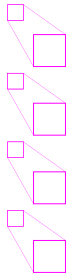
\includegraphics[width=0.135\linewidth]{figs/SR/Bicubic}
    }
    \subfloat[Baseline]{
        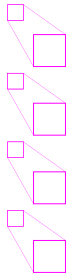
\includegraphics[width=0.135\linewidth]{figs/SR/Photography}
        \label{figure:comparisons/baseline}
    }
    \subfloat[Ours (MAE)]{
        \includegraphics[width=0.135\linewidth]{figs/SR/Ours@ESPCN@L1}
        \label{figure:comparisons/mae}
    }
    \subfloat[Ours (MSE)]{
        \includegraphics[width=0.135\linewidth]{figs/SR/Ours@ESPCN@L2}
        \label{figure:comparisons/mse}
    }
    \smallbreak
    \subfloat[Ours (DSSIM)]{
        \includegraphics[width=0.135\linewidth]{figs/SR/Ours@ESPCN@SSIM}
        \label{figure:comparisons/dssim}
    }
    \subfloat[Ours (MS-DSSIM)]{
        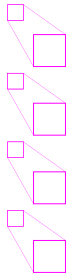
\includegraphics[width=0.135\linewidth]{figs/SR/Ours@ESPCN@MS-SSIM}
        \label{figure:comparisons/ms-dssim}
    }
    \subfloat[Ours (MixGE)]{
        \includegraphics[width=0.135\linewidth]{figs/SR/Ours@ESPCN@Sobel001}
        \label{figure:comparisons/mixge}
    }
    \subfloat[Ours (Sketch)]{
        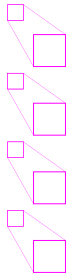
\includegraphics[width=0.135\linewidth]{figs/SR/Ours@ESPCN@Sketch}
        \label{figure:comparisons/sketch}
    }
    \subfloat[Ours (Perceptual)]{
        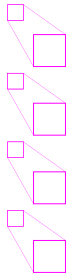
\includegraphics[width=0.135\linewidth]{figs/SR/Ours@ESPCN@Perceptual}
        \label{figure:comparisons/perceptual}
    }

    \caption[]{
        Comparison across loss functions on the \textbf{Small} network.
        Regions outlined in magenta are magnified to better visualize the impact of applying different SISR methods. ``Ours (MixGE)'' uses $\lambda_G = 0.01$ and the Baseline is the pre-trained Y-channel ESPCN model.
        From top to bottom rows, images are cropped samples of the following sources:
        \begin{enumerate*}
            \item Manga109\cite{mtap_matsui_2017,multimedia_aizawa_2020}, \copyright~Ken~Akamatsu\label{figure:manga109}
            \item Wikipedia (\url{https://en.wikipedia.org/wiki/File:Wikipe-tan_face.svg})
            \item SYNLA dataset\cite{synla}
            \item Set14 dataset\cite{zeyde2010single}.
        \end{enumerate*}
    }

    \label{figure:comparisons}
\end{figure*}



\begin{figure*}[h!]
    \centering

    \subfloat[Input]{
        \includegraphics[width=0.11\linewidth]{figs/SR/LR}
    }
    \subfloat[Ground Truth]{
        \includegraphics[width=0.11\linewidth]{figs/SR/HR}
    }
    \subfloat[MAE]{
        \includegraphics[width=0.11\linewidth]{figs/SR/Ours@Residual@L1}
    }
    \subfloat[MSE]{
        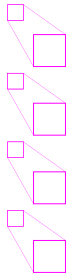
\includegraphics[width=0.11\linewidth]{figs/SR/Ours@Residual@L2}
        \label{figure:comparisons/large/mse}
    }
    \subfloat[SSIM]{
        \includegraphics[width=0.11\linewidth]{figs/SR/Ours@Residual@SSIM}
    }
    \subfloat[MS-SSIM]{
        \includegraphics[width=0.11\linewidth]{figs/SR/Ours@Residual@MS-SSIM}
    }
    \subfloat[Perceptual]{
        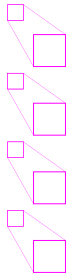
\includegraphics[width=0.11\linewidth]{figs/SR/Ours@Residual@Perceptual}
    }
    \subfloat[MixGE]{
        \includegraphics[width=0.11\linewidth]{figs/SR/Ours@Residual@Sobel}
    }
    \caption{
        Comparison across loss functions on our \textbf{Large} network. See Figure~\ref{figure:comparisons} for image sources.
    }

    \label{figure:comparisons-large}
\end{figure*}


In this section, we discuss the results obtained from training the neural networks with the loss functions discussed through the work, presented in Table~\ref{table:quantitative}. We also present a few handpicked samples in Figure~\ref{figure:comparisons} and Figure~\ref{figure:comparisons-large} for discussion as part of our qualitative analysis. 

Two images which did not originate from the datasets listed in Section~\ref{section:datasets} were included for qualitative analysis: the image in the fourth row is an illustration frequently used as a test case across super-resolution works. The level of details in this image reduces the gap between the result obtained from the baseline network (Figure~\ref{figure:comparisons/baseline}) and our best result (Figure~\ref{figure:comparisons/mixge}). \adding{The image in the second row was included as a sample vectorial illustration image, allowing the generation of a low-resolution input without downsampling artifacts.}

\subsection{Analysis on the small network}

From experimental observations, the $\MAE$ caused the training process to reach a plateau after the least number of iterations among the studied functions, followed by the Pencil Sketch, $\DSSIM$. The training process persisted for the $\MSE$, the $\MSDSSIM$, the perceptual loss and the mixed gradient error until the upper limit of 1500 epochs.

While the images produced by the network trained with the MAE loss have less noise than the one trained with the MSE, it has caused aliased edges in flat images, such as the second row in Figure~\ref{figure:comparisons/mae}, motivating further exploration.

It was observed that the DSSIM led the network to optimize for edge restoration at the expense of accuracy in color reproduction.
In the second row of Figure~\ref{figure:comparisons/dssim}, the image has less noise than its counterparts, but the colorization of the character is visibly different.
This can also be observed in the first row: the image has a slight red hue compared to its grayscale counterparts.
While this did not occur in the network trained with the $\MSDSSIM$ loss (Figure~\ref{figure:comparisons/ms-dssim}), the images produced by it are also noisier.

\begin{figure}[htbp]
    \centering

    \subfloat[MixGE]{
        \includegraphics[width=0.45\linewidth]{figs/SR/Wikipe-tan/Ours@ESPCN@Sobel001}
        \label{fig:comparison/wiki-ours}
    }
    \subfloat[Baseline]{
        \includegraphics[width=0.45\linewidth]{figs/SR/Wikipe-tan/Photography}
        \label{fig:comparison/wiki-photo}
    }
    \smallbreak
    \subfloat[MixGE]{
        \includegraphics[width=0.45\linewidth]{figs/SR/SYNLA@Color/Ours@ESPCN@Sobel001}
        \label{fig:comparison/synla-ours}
    }
    \subfloat[Baseline]{
        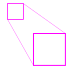
\includegraphics[width=0.45\linewidth]{figs/SR/SYNLA@Color/Photography}
        \label{fig:comparison/synla-photo}
    }

    \caption{
        \label{fig:comparison}
        Comparison of the photography-centric baseline against the small network trained with the MixGE loss ($\lambda_G = 0.01$).
        Figure~\ref{fig:comparison/wiki-ours} depicts a case where the neural network trained on the gradient loss produces smoother edges.
        Figure~\ref{fig:comparison/synla-ours} depicts a pathological case with excessive production of noise.
    }
\end{figure}

As seen in Table~\ref{table:quantitative}, variations of the MixGE loss function have led to the best results in most recorded metrics. While it has been observed to reconstruct well in general scenarios, images restored from blurry low-resolution pictures, such as the image in the second row in Figure~\ref{figure:comparisons}, have shown the highest incidence of noise among the trained networks, as seen in Figure~\ref{fig:comparison}, characterizing a pathological case.

Our experiments showed little to no impact in assigning three different weights ($0.01$, $0.10$, $1.00$) to the $\lambda_G$ gradient component of the MixGE loss --- as seen in Table~\ref{table:quantitative}, metric results were close to each other and no discernible differences were observed in an analysis of the reconstructed images.

Despite their similar formulation, the Pencil Sketch loss function (Figure~\ref{figure:comparisons/sketch}) did not show comparable performance to the Mixed Gradient Error, having substantially lower scores across the board and producing noisier images.
We also found this loss function to be inherently unstable during the training, sometimes causing divisions by zero despite the stabilizing term. This instability may be attributed to the network output being unconstrained: during the early stages of training, a randomly initialized network can produce values which causes a division by zero in Equation~\ref{equation:sketch}, despite the stabilizing term $\epsilon$, making this loss function unsuitable for such cases.

The Perceptual Loss (Figure~\ref{figure:comparisons/perceptual}) has shown similar quality characteristics as the Mixed Gradient Error: in images with solid regions, it produces less noise than the alternatives while producing more of such artifacts in blurry images.

We also observed that the depth of the chosen feature descriptor $\phi$ entails a trade-off: a shallow descriptor may optimize only for lower-level features, such as drawing primitives, while a deep descriptor may discard details deemed unnecessary to the task for which it was previously trained, potentially causing undesirable artifacts, as seen in Figure~\ref{figure:perceptual/comparison}. 
This was explored through the inclusion and omission of a pooling layer in the feature descriptor: because the noise information is discarded by the feature extractor with the pooling, it is not back-propagated, causing the reconstructed image in Figure~\ref{figure:perceptual/with-maxpool} to be unconstrained and have artifacts that would otherwise not be present, as in Figure~\ref{figure:perceptual/without-maxpool}.

\begin{figure}[htbp]
    \centering
    \label{figure:perceptual/comparison}

    \subfloat[\label{figure:perceptual/without-maxpool}Without Max Pooling]{
        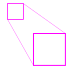
\includegraphics[width=0.45\linewidth]{figs/perceptual/BeforeMaxPool}
    }
    \subfloat[\label{figure:perceptual/with-maxpool}With Max Pooling]{
        \includegraphics[width=0.45\linewidth]{figs/perceptual/AfterMaxPool}
    }
    \caption{
        Effects of the inclusion and omission of a pooling operation in a feature descriptor.
    }
\end{figure}

Regarding the modifications applied to the ESPCN architecture, we observe that the addition of the non-parametric normalization layer at the start of the network helped the training process by making the model to learn faster.

\subsection{\label{section:analysis-large-network}Analysis on the large network}

In regards to the larger network, three factors that particularly stand out in Table~\ref{table:quantitative} and in Figure~\ref{figure:comparisons-large} are described in this section.

The Mean Squared Error network yielded substantially worse results than all of the other large networks, producing a large amount of noise artifacts in the images, shown in Figure~\ref{figure:comparisons/large/mse}. This has caused the network to produce results with worse visual quality than the ones produced by the small network (Figure~\ref{figure:comparisons}), despite higher metric scores.

Contrary to our previous expectations that a loss function would retain its performance characteristics across network size, Table~\ref{table:quantitative} shows that this may not be true in practice: the Structural Dissimilarity and the Mean Absolute Error, which performed poorly on the smaller network, yielded the best metric results.

With exception of the Mean Squared Error and the Multi-scale Structural Similarity networks, most results are visually indistinguishable. This could be explained by considering that a sufficiently large network may be able to learn all of the characteristics of a training dataset, rendering the intrinsic prioritization of a loss function redundant.

\section{Conclusions}

Through the analysis of the experimental evaluation, we observed significant improvements in the super-resolution task by applying the domain knowledge in the loss function of a \adding{small} neural network. Within the context of this work, the knowledge that illustrations generally emphasize edges was used in order to search for a loss function more apt to consider this factor.
However, the best network showed pathological behavior over certain types of images, \eg, an originally blurred image.

\adding{
    However, on larger networks, the choice of a loss function was not as impactful as originally expected. This result may provide further motivation for why the mean squared error is considered the ``default'' choice, in addition to its direct relation to the PSNR metric (Equation~\ref{equation:psnr}).

    Also unexpectedly, it was observed that the ordering of loss function performances may not be maintained across network sizes: in this work, two of the worst losses in a small network (mean absolute error, structural dissimilarity) led to the best results in the large network. Exploring what causes this is a possible topic for future works.
}

Motivated by the fact that some loss functions perform better on some types of illustrations, which encompasses line art to drawings with rich textures, future works may benefit a stricter segregation by image types of the test dataset.

Moreover, our work did not explore complex loss functions, such as combinations of losses, nor GANs, leaving room for improvement.

\subsection*{Acknowledgments}

The authors would like to thank CAPES, CNPq and FAPEMIG agencies for supporting this project.

\bibliographystyle{IEEEtran}
\bibliography{example}

\end{document}